% Gallery figure source
% Summary: A recombinant alignment can be read as a sequence of genome intervals, each with its own local tree. Dashed guide lines connect each local-tree tip to the corresponding sampled genome row. The colors mark intervals, not observed nucleotides.
\documentclass[tikz,border=6pt]{standalone}
% Shared color palette
\usepackage[T1]{fontenc}
\usepackage[utf8]{inputenc}
\usepackage{lmodern}
\usepackage{microtype}
\usepackage{amsmath,amssymb,mathtools}
\usepackage{xcolor}
\usepackage{tikz}
\usetikzlibrary{arrows.meta,positioning,calc,fit,backgrounds,decorations.pathreplacing,shapes.geometric,shadows.blur}

\definecolor{mainblue}{RGB}{42,85,132}
\definecolor{deepgreen}{RGB}{30,105,70}
\definecolor{burntorange}{RGB}{190,90,25}
\definecolor{softgray}{RGB}{245,246,248}
\definecolor{darkgray}{RGB}{70,70,70}
\definecolor{violet}{RGB}{110,70,150}

\newcommand{\given}{\,|\,}
\newcommand{\Ne}{N_{e}}
\newcommand{\ARG}{\mathrm{ARG}}
\newcommand{\MRCA}{\mathrm{MRCA}}
\newcommand{\GMRCA}{\mathrm{GMRCA}}

% Shared TikZ styles
\tikzset{
  tip/.style={circle,fill=black,inner sep=1.6pt},
  nodept/.style={circle,fill=black,inner sep=1.4pt},
  sampled/.style={rectangle,fill=black,inner sep=2.2pt},
  branch/.style={line width=0.8pt},
  retic/.style={circle,draw=burntorange,fill=burntorange!25,line width=0.8pt,inner sep=2.0pt},
  event/.style={circle,draw=mainblue,fill=mainblue!15,line width=0.8pt,inner sep=1.8pt},
  arr/.style={-{Latex[length=2.0mm]},line width=0.8pt},
  faint/.style={line width=0.7pt,draw=gray!55},
  parentedge/.style={-{Latex[length=2.0mm]},line width=0.9pt,draw=burntorange},
  treeedge/.style={-{Latex[length=2.0mm]},line width=0.9pt,draw=black},
  segment/.style={line width=4pt,line cap=round},
  dashedretic/.style={-{Latex[length=2.0mm]},line width=0.9pt,draw=burntorange,dashed}
}


\begin{document}
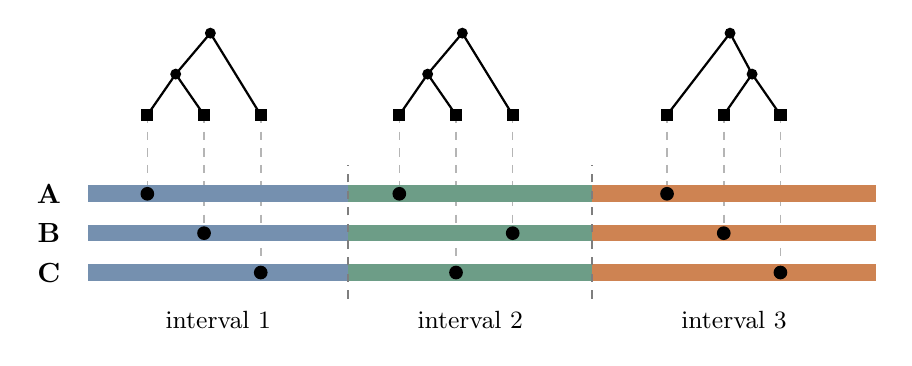
\begin{tikzpicture}[
  scale=1.0,
  genomebar/.style={line width=6pt,line cap=butt},
  guide/.style={line width=.55pt,dashed,draw=gray!58},
  boundary/.style={line width=.65pt,dashed,draw=darkgray!70},
  joint/.style={circle,fill=black,inner sep=1.75pt},
  treelabel/.style={font=\scriptsize,text=darkgray,align=center}
]

  \coordinate (rowAref) at (0,0.35);
  \coordinate (rowBref) at (0,-0.15);
  \coordinate (rowCref) at (0,-0.65);

  \begin{scope}[xshift=1.55cm,yshift=1.35cm,scale=0.8]
    \coordinate (t1r) at (1.0,1.3);
    \coordinate (t1n) at (0.45,0.65);
    \coordinate (t1A) at (0.0,0);
    \coordinate (t1B) at (0.9,0);
    \coordinate (t1C) at (1.8,0);

    \draw[branch] (t1r)--(t1n)--(t1A);
    \draw[branch] (t1n)--(t1B);
    \draw[branch] (t1r)--(t1C);

    \foreach \p in {t1r,t1n}{
      \node[nodept] at (\p) {};
    }
  \end{scope}

  \begin{scope}[xshift=4.75cm,yshift=1.35cm,scale=0.8]
    \coordinate (t2r) at (1.0,1.3);
    \coordinate (t2n) at (0.45,0.65);
    \coordinate (t2A) at (0.0,0);
    \coordinate (t2C) at (0.9,0);
    \coordinate (t2B) at (1.8,0);

    \draw[branch] (t2r)--(t2n)--(t2A);
    \draw[branch] (t2n)--(t2C);
    \draw[branch] (t2r)--(t2B);

    \foreach \p in {t2r,t2n}{
      \node[nodept] at (\p) {};
    }
  \end{scope}

  \begin{scope}[xshift=8.15cm,yshift=1.35cm,scale=0.8]
    \coordinate (t3r) at (1.0,1.3);
    \coordinate (t3n) at (1.35,0.65);
    \coordinate (t3A) at (0.0,0);
    \coordinate (t3B) at (0.9,0);
    \coordinate (t3C) at (1.8,0);

    \draw[branch] (t3r)--(t3A);
    \draw[branch] (t3r)--(t3n)--(t3B);
    \draw[branch] (t3n)--(t3C);

    \foreach \p in {t3r,t3n}{
      \node[nodept] at (\p) {};
    }
  \end{scope}

  \draw[guide] (t1A) -- (t1A |- rowAref);
  \draw[guide] (t1B) -- (t1B |- rowBref);
  \draw[guide] (t1C) -- (t1C |- rowCref);

  \draw[guide] (t2A) -- (t2A |- rowAref);
  \draw[guide] (t2B) -- (t2B |- rowBref);
  \draw[guide] (t2C) -- (t2C |- rowCref);

  \draw[guide] (t3A) -- (t3A |- rowAref);
  \draw[guide] (t3B) -- (t3B |- rowBref);
  \draw[guide] (t3C) -- (t3C |- rowCref);

  \node[font=\bfseries] at (0.3,0.35) {A};
  \node[font=\bfseries] at (0.3,-0.15) {B};
  \node[font=\bfseries] at (0.3,-0.65) {C};

  \foreach \y in {0.35,-0.15,-0.65}{
    \draw[genomebar,draw=mainblue!65] (0.8,\y)--(4.1,\y);
    \draw[genomebar,draw=deepgreen!65] (4.1,\y)--(7.2,\y);
    \draw[genomebar,draw=burntorange!75] (7.2,\y)--(10.8,\y);
  }

  \draw[boundary] (4.1,-0.98)--(4.1,0.72);
  \draw[boundary] (7.2,-0.98)--(7.2,0.72);

  \node[font=\small] at (2.45,-1.25) {interval 1};
  \node[font=\small] at (5.65,-1.25) {interval 2};
  \node[font=\small] at (9.0,-1.25) {interval 3};

  \foreach \p in {t1A,t1B,t1C,t2A,t2B,t2C,t3A,t3B,t3C}{
    \node[sampled] at (\p) {};
  }

  \node[joint] at (t1A |- rowAref) {};
  \node[joint] at (t1B |- rowBref) {};
  \node[joint] at (t1C |- rowCref) {};

  \node[joint] at (t2A |- rowAref) {};
  \node[joint] at (t2B |- rowBref) {};
  \node[joint] at (t2C |- rowCref) {};

  \node[joint] at (t3A |- rowAref) {};
  \node[joint] at (t3B |- rowBref) {};
  \node[joint] at (t3C |- rowCref) {};

\end{tikzpicture}
\end{document}
